\chapter{Patrones}
\section{Introducción}
Aunque históricamente el software pueda considerarse como primitivo si se compara con otras disciplinas que llevan siglos de ventaja en cuanto a su desarrollo, actualmente no es así. La anterior reflexión se deduce debido a que el software ha evolucionado lo suficiente para convertirse en una herramienta que va mas allá de solo programar, también se encarga de diseñar y modelar. En este caso, el diseño de software puede generar soluciones generalizadas a problemas reincidentes. Así es como llegamos a los patrones de diseño, los cuales para cualquier proyecto, independientemente de su complejidad y tamaño, seguramente se verán involucrados.

A partir de lo anterior, es claro que los patrones de diseño aparecerán en la propuesta de estructura del proyeto, más conocida como diagrama de clases, con la intención de obtener un diagrama razonable desde un punto de vista de principios de diseño así como los principios del paradigma orientado a objetos. 

Se debe mencionar también que los patrones propuestos en este documento, no necesariamente todos están incluidos en el Gof (the Gang of Four), pues existen otras soluciones que aunque no tan conocidas, pueden tener un impacto positivo debido en el desarrollo del software.
\newpage

\section{Composite}
El patrón de diseño Composite (Componente), nos permite construir estructuras complejas partiendo de otras estructuras mucho mas simples, lo cual permite crear estructuras compuestas conformadas por otras mas pequeñas. Este patrón resulta útil para la creación de subtareas dentro de una tarea mas general, ya que se genera una estructura en forma de árbol gracias a la recursividad con la que funciona el patrón. Otra ventaja de su utilización, en este desarrollo específicamente,  es que se puede representar la jerarquía de tarea-subtarea, además de añadir dinamismo a la tarea, ya que ésta puede tener subtareas de diferentes tipos. Además es posible tratar la subtarea como tarea.
\\
En conclusión, el patrón componente posibilita la solución del problema de las subtareas, ya que permite jerarquizar, añadir dinamismo a la tarea por medio de subtareas y construir la tarea general por medio de subtareas, por esta razón será utilizado dentro de este software.

\begin{figure}[H]
	\centering
	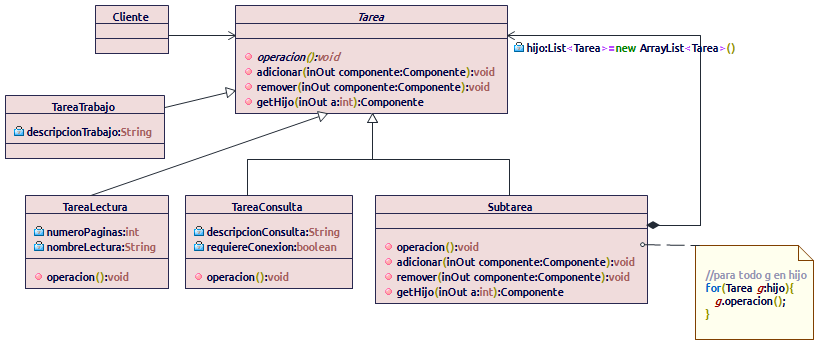
\includegraphics[width=1\linewidth]{diseno/patrones/imgs/Composite}
	\caption{Patrón Componente}
	\label{fig:gantt}
\end{figure}

\section{Agrupación}
Un horario puede mostrarse como la constitución de diversas franjas en un orden lógico; estas deben agruparse para que haya orden y se puedan manejar conjuntamente. Por está razón el patrón agrupación será de utilidad, ya que permite generar una estructura en la cual los módulos, que en este caso son las franjas, puedan ser agrupados para invocarse de forma colectiva como el horario, de esta forma se centraliza el control de la estructura en una sola clase.

\begin{figure}[H]
	\centering
	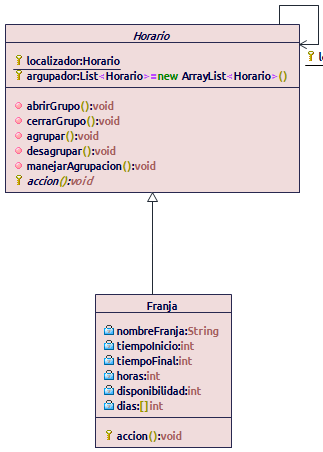
\includegraphics[width=0.5\linewidth]{diseno/patrones/imgs/Agrupador}
	\caption{Patrón Agrupador}
	\label{fig:gantt}
\end{figure}

\section{Patrón Fábrica Abstracta}
La creación de objetos es una situación que aparece en prácticamente cualquier proyecto, por lo que se debe buscar una estructura que permita llevar esta creación de la mejor manera, incluso en mayor medida cuando el objeto a crear pertenece a una familia de otros objetos que también pueden ser creados, y por supuesto en un caso más general en caso de que hayan varias de estas familias de objetos.

La fábrica abstracta lo que hace es esto, proveer una interfaz para la creación de estas familias de objetos relacionados, sin especificar sus clases concretas.

Para el caso del proyecto, la fábrica abstracta es útil pues existen dos familias de objetos a crear, una de tareas referente a lo académico y otra la de tareas que no tienen que ver con la universidad.

\begin{figure}[H]
	\centering
	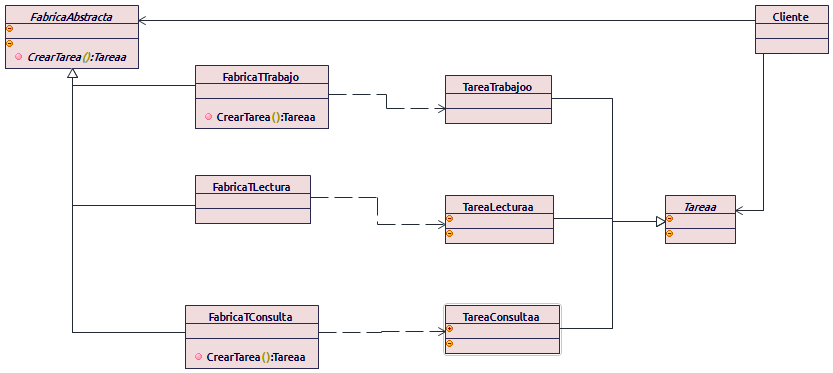
\includegraphics[width=1\linewidth]{diseno/patrones/imgs/FabricaAbstracta}
	\caption{Patrón Fábrica Abstracta}
	\label{fig:gantt}
\end{figure}

\section{Patrón Estrategia}
Dada la situación de que un programa pueda ofrecer un servicio, el cual se pueda realizar de varias maneras hace alusión a este patrón. La intención de este es poder seleccionar la alternativa más adecuada para el cliente, durante tiempo de ejecución.

En la mención a la fábrica abstracta se mencionaron las familias de objetos de tarea y categoria, las cuales en algún momento necesitarán de la posibilidad de una modificación de alguno de sus objetos, operación que no solo involucra a este último en cuestión, sino que abarca principalmente el modulo externo de manejo de base de datos. Dependiendo de cada objeto, la misma operación debe hacerce de manera distinta, haciendo así que entre el patrón estrategia.

\begin{figure}[H]
	\centering
	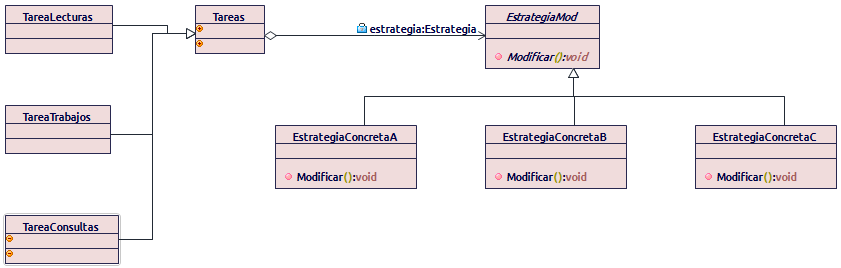
\includegraphics[width=1\linewidth]{diseno/patrones/imgs/Estrategia}
	\caption{Patrón Estrategia}
	\label{fig:gantt}
\end{figure}

Código fuente, clase Horario:

\begin{lstlisting}[language = Java  , firstnumber = last , escapeinside={(*@}{@*)}]
import java.util.List;
import java.util.ArrayList;
public abstract class Horario{
	protected static Horario localizador;
	protected List<Horario> argupador=new ArrayList<Horario>();
	public static void main(String[] args){
		Horario A =  new Franja();
		A.abrirGrupo();
		A.agrupar();
		A.manejarAgrupacion();
		Horario B =  new AgrupadorB();
		B.agrupar();
		B.manejarAgrupacion();
	}
	public void abrirGrupo(){
		if(localizador==null){
   			localizador=this;
   			argupador=new ArrayList<Horario>();
   		}
	}
	public void cerrarGrupo(){
		localizador = null;
	}
	public void agrupar(){
		if(localizador!=null){
   			(argupador = localizador.argupador).add(this);
		}
	}
	public void desagrupar(){
		if(localizador!=null){
   			localizador.argupador.remove(this);
		}
	}
	public void manejarAgrupacion(){
		for(Horario a:argupador){
 	    	a.accion();
		}
	}
	protected abstract void accion();
}
\end{lstlisting}

Código fuente, clase Franja:
\begin{lstlisting}[language = Java  , firstnumber = last , escapeinside={(*@}{@*)}]
import static com.componentes.diseno.lmc.marcosDeReferencia.computacion.Computacion.*;
import static com.componentes.diseno.lmc.marcosDeReferencia.emoticons.Emoticons.*;
public class Franja extends Horario{
	private String nombreFranja;
	private int tiempoInicio;
	private int tiempoFinal;
	private int horas;
	private int disponibilidad;
	private []int dias;
	protected void accion(){
		System.out.println(SERIOUS);
	}
}
\end{lstlisting}